\documentclass[preview]{standalone}

\usepackage{tikz}

\begin{document}
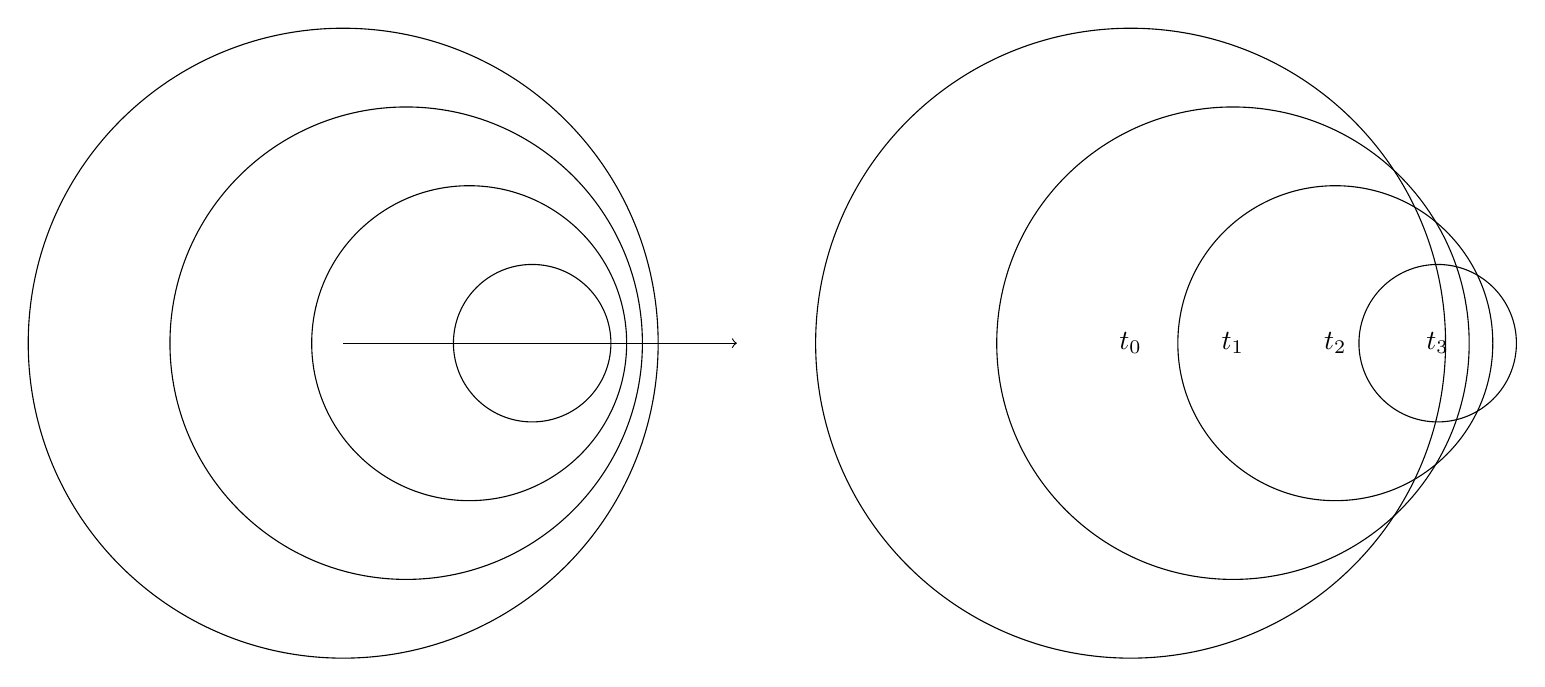
\begin{tikzpicture}
   % c = 1, what else

   \draw[->] (0,0) -- (5,0);
   \foreach \t in {0,...,3} {
     \node (X) at (0.8*\t,0) {};
     \draw (X) circle[radius=(4-\t)];
   }
   \foreach \t in {0,...,3} {
     \node (X) at (10 + 1.3*\t,0) {$t_\t$};
     \draw (X) circle[radius=(4-\t)];
   }
\end{tikzpicture}
\end{document}
